\section{Résultats} % (fold)
\label{sec:résultats}

\paragraph{Tests préliminaires} % (fold)
\label{par:tests_pr_liminaires}
Sur les 62 échantillons testés, 44 étaient effectivement infectés par \esp{Wolbachia}, et ont donc été typés en transposon-display.
% paragraph tests_pr_liminaires (end)

\paragraph{Polymorphismes} % (fold)
\label{par:polymorphisme}
Nous retrouvons des profils similaires à ceux déjà obtenus auparavant\cite{memHH}, enrichis de nouvelles lignées pour les espèces déjà typées en transposon-display, et d'espèces typées pour la première fois, comme \esp{D. auraria}, \esp{D. triauraria} et \esp{D. suzukii}. % D.sub aussi
La figure \ref{fig:profils} montre un exemple de chaque profil différent.

\begin{figure}[h]
	\begin{center}
		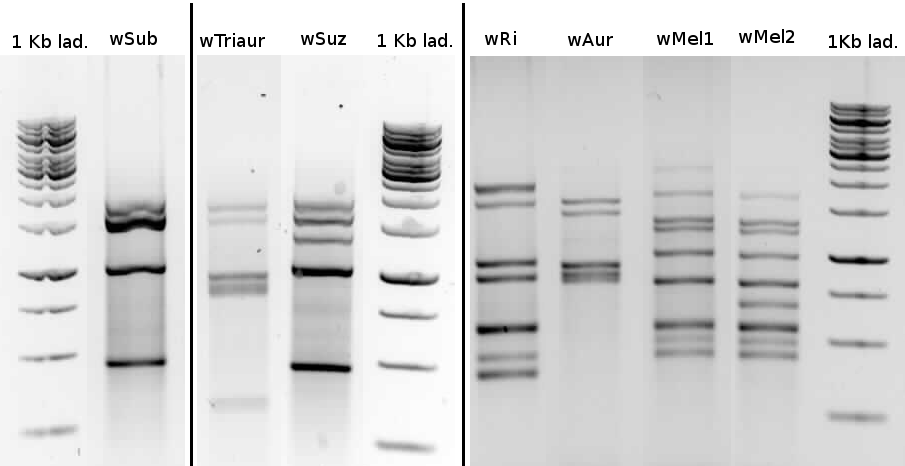
\includegraphics[width=150mm]{images/profils_crop.png}
	\end{center}
	\caption{Reconstruction d'un gel représentant tous les profils caractéristiques des souches de \esp{Wolbachia} en transposon-display avec les amorces Isb/LNP.}
	\label{fig:profils}
\end{figure}

Pour les nouvelles souches passées en transposon-display, nous pouvons faire les observations suivantes : 
\begin{enumerate}
	\item \esp{wTriaur} et \esp{wAur} ont des profils similaires, ce qui peut s'expliquer par la très forte apparenté de ses hôtes.
	\item De la même façon, \esp{wSub} semble partager beaucoup fragments avec \esp{wSuz}, témoin aussi d'une forte apparenté de ses hôtes.\\
	\esp{wSuz} de son coté forme un groupe très homogène, avec un profil spécifique.
	\item Une souche de \esp{wMel} issue d'une lignée de Madagascar présente un fragment supplémentaire (wMel2 sur la figure \ref{fig:profils}).\\
	\esp{wMel} constituait jusqu'à présent un groupe très homogène.
	Un échantillonnage supplémentaire devra donc être fait dans les lignées de \esp{wMel}, notamment celles provenant de Madagascar.
	\item \esp{wRi} reste toujours un groupe bien homogène au sein de \esp{D. simulans}.
\end{enumerate}


% paragraph polymorphisme (end)

\paragraph{Une amélioration nette du protocole.} % (fold)
\label{par:proto}
Un des éléments notables dans les gels d'électrophorèse obtenus est la nette amélioration de l'amplification des fragments de grande taille, notamment pour les profils de type \textit{wMel} (Cf. Figure \ref{fig:wMelcomp}). 

\begin{figure}[h]
	\begin{center}
		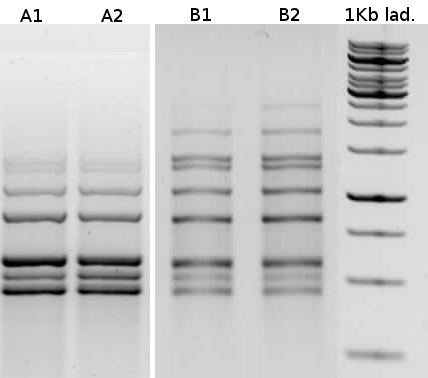
\includegraphics[width=80mm]{images/wMel_comp.png}
	\end{center}
	\caption{Comparaison des deux protocoles sur wMel (\esp{Wolbachia} de \esp{D. melanogaster})~:
	A1 et A2 : Ancien protocole\cite{memHH}~;
	B1 et B2 : Nouveau protocole, avec accuTaq}
	\label{fig:wMelcomp}
\end{figure}

% paragraph proto (end)
% section r_sultats (end)

\section{Discussions \& Perspectives} % (fold)
\label{sec:discussions}

\paragraph{wRi-like} % (fold)
\label{par:wri_like}
On observe toujours une dichotomie au sein du groupe \esp{wRi-like}\footnote{Les \esp{wRi-like} comprennent, pour rappel, les bactéries de la drosophile \esp{D. simulans} (\esp{wRi}) et celles de \esp{D. auraria} et associées.}. La bactérie de \esp{D. triauraria} présentant un profil de type \esp{wAur}.
% paragraph wri_like (end)

\paragraph{wMel-like} % (fold)
\label{par:wmel_like}
Les bactéries du groupe \esp{wMel-like} présentent toujours une bonne homogénéité sur la base de ce marqueur, excepté pour une lignée provenant de Madagascar, qui présente un fragment de plus, d'environ 700 paires de bases.
% paragraph wmel_like (end)

\paragraph{Un nouveau profil : «\textit{wSuz-like}»} % (fold)
\label{par:suzukii}
Un nouveau profil semble se dégager, regroupant les bactéries de \esp{D. suzukii} et celles de sa proche parente \esp{D. subpulchrella}. Elles semblent tout du moins différer d'un fragment, d'environ 1\,500 paires de bases.
% paragraph un_nouveau_profil_wsuz-like_ (end)

\paragraph{Perspectives\\} % (fold)
\label{par:perspectives}
Outre la nécessité de typer encore plus d'échantillons (notamment pour confirmer le nouveau profil des \esp{wMel} malgaches),
la prochaine étape de cette étude serait de séquencer les fragments obtenus avec le transposon-display, et ce dans deux buts~:
Tout d'abord pour confirmer les égalités entre bandes, que nous n'affirmons pour l'instant que de façon visuelle.

Ensuite, ces séquençages nous permettraient situer les insertions dans le génome complet, grâce aux régions flanquantes. 
Nous pourrions donc identifier les gènes qui ont été inactivés par cette insertion. Peut-être aurons-nous des informations fonctionnelles expliquant en partie la réussite du transfert horizontal pour ces cas particulier.

\paragraph{} % (fold)
\label{par:vide}
Pour finir, nous pourrions dans une vision à plus long terme envisager des études similaires sur d'autres marqueurs qu'ISWpi1, choisi certes pour sa spécificité pour \esp{Wolbachia}, mais aussi parce qu'il est à l'heure actuelle, le plus décrit dans la littérature. Cela nous permettrait d'accroître encore d'avantage la résolution de notre vision des micro-évolutions au sein de ce groupe.
% paragraph  (end)
% paragraph perspectives (end)


